\chapter{पादप जीवन: जड़ जमाए हुए फलना-फूलना}\label{ch:g12:plant-rooted-life}

कोई बलूत पानी तक चलकर नहीं जा सकता, किसी इल्ली से भाग नहीं सकता, न किसी
साथी की तलाश में निकल सकता है। वह तीन सदियों तक वहीं खड़ा रहता है जहाँ उसका
बलूत-फल गिरा था, और उस दौरान वह मिट्टी से सैकड़ों टन पानी उठाता है, उसे खा
जाने को तैयार हज़ारों \omterm{def:g10:biodiversity-scales:species}{जातियों} को दूर रखता है, प्रकाश के पीछे चलने के लिए
अपने पत्ते घुमाता है, और अपना पराग तथा अपने बलूत-फल हवा से और जे पक्षियों से
देहात भर भेजता है। जड़ जमाया जीवन कोई निष्क्रिय जीवन नहीं है; वह उन्हीं
समस्याओं --- खाना, बचाव, हिलना, जनन --- के हलों का एक अलग समुच्चय है, और यह
अध्याय उन्हीं का सर्वेक्षण करता है।

\section{लेन-देन के लिए बनी एक देह}

\begin{proposition}[दो तंत्र, दो सतहें]\label{prop:g12:plant-rooted-life:surfaces}
कोई फूल वाला पौधा दो तंत्रों में व्यवस्थित है: मिट्टी में \emph{मूल तंत्र},
जो पानी तथा खनिज आयन सोखता है और उस पौधे को गाड़े रखता है, और हवा में
\emph{प्ररोह तंत्र} --- यानी तने और पत्ते --- जो प्रकाश तथा कार्बन
डाइऑक्साइड पकड़ता है। हर एक लेन-देन की एक विशाल सतह है: किसी बड़े पेड़ के
पत्ते प्रकाश के सामने कई सौ वर्ग मीटर सतह फैलाते हैं, और उसकी जड़ें, जो
अरबों सूक्ष्म \emph{मूलरोमों}\index{मूलरोम} से बढ़ाई गई हैं, मिट्टी के सामने
कई सौ वर्ग मीटर। कोई पौधा सबसे बढ़कर किसी नियत बिंदु से दो दिशाओं में सतह
फैलाने का एक ढंग है।
\end{proposition}
\begin{proof}[साक्ष्य]
मिट्टी के किसी डिब्बे में चार महीने उगाए गए राई के एक ही पौधे में
$\num{1.4e10}$ \omterm{prop:g12:plant-rooted-life:surfaces}{मूलरोम} पाए गए, जिनकी कुल लंबाई \qty{10000}{km} से ऊपर और
सतह लगभग \qty{400}{m^2} थी, यानी उसके पत्तों की सतह से दस गुनी। कोई पूरा
बढ़ा बलूत कोई 250\,000 पत्ते ढोता है; और जंगल का एक हेक्टेयर आसमान के
सामने \qtyrange{5}{8}{ha} पत्ती सतह पेश करता है। किसी नन्हे पौधे के \omterm{prop:g12:plant-rooted-life:surfaces}{मूलरोम}
काट देने पर, या उसके पत्तों पर परत चढ़ा देने पर, उसकी बढ़त दिनों में रुक
जाती है।
\end{proof}

\begin{omfigure}
\begin{tikzpicture}
  \node[anchor=south west, inner sep=0] (img) at (0,0)
    {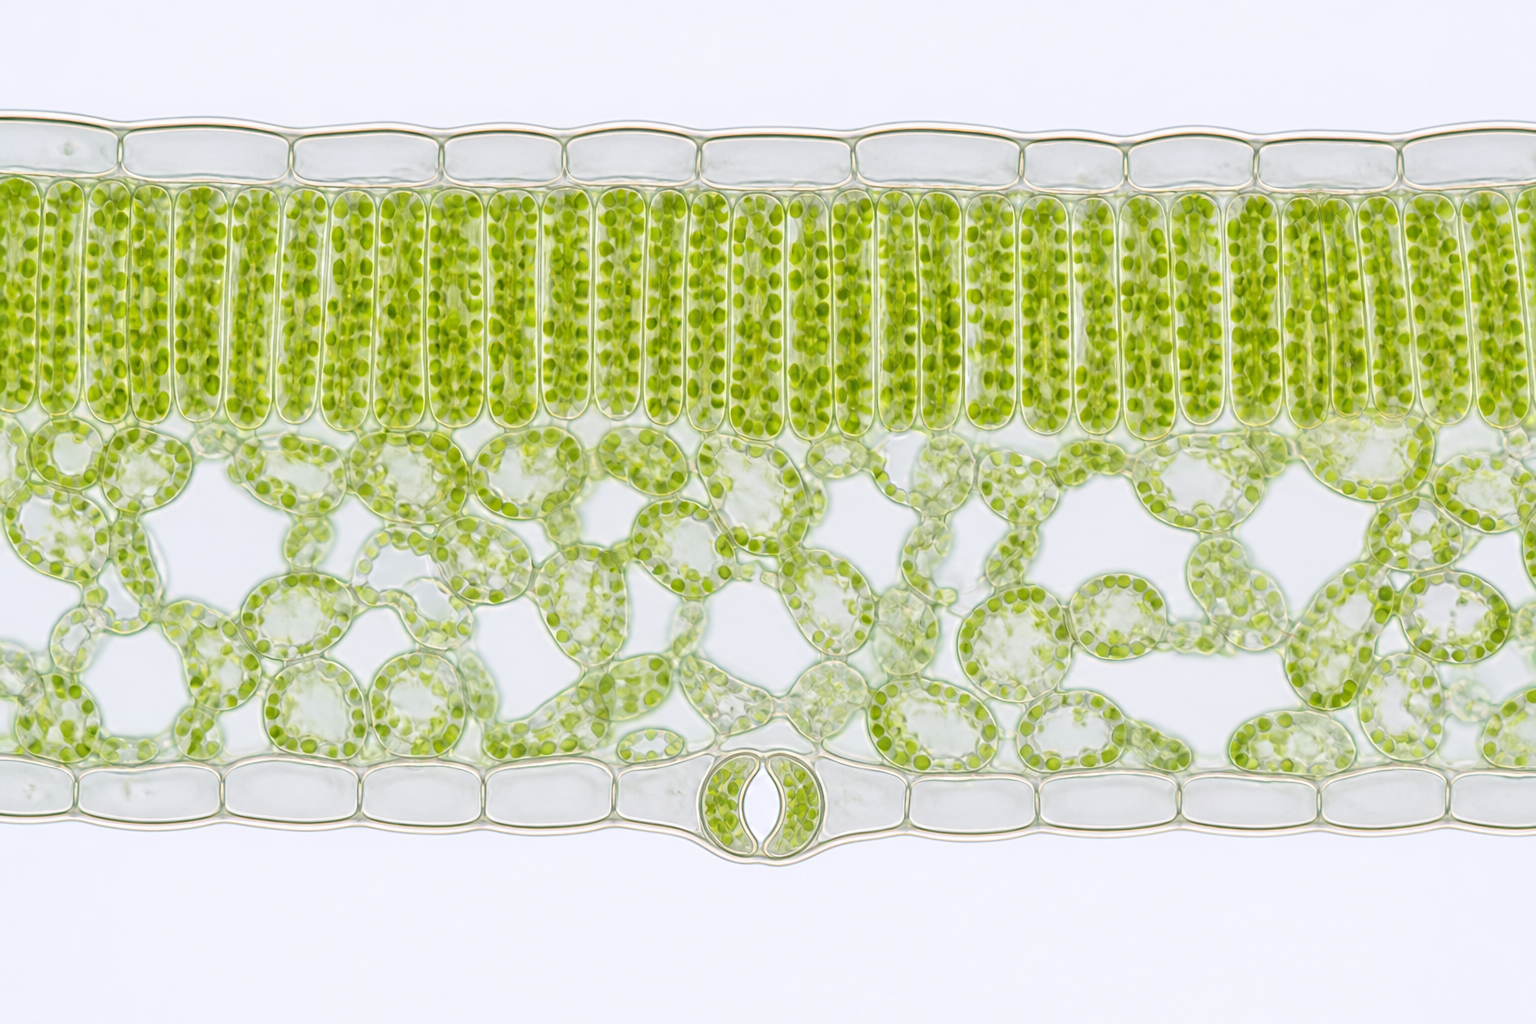
\includegraphics[width=0.56\linewidth]{images/book2/ai/fig-leaf-cross-section.png}};
  \begin{scope}[x={(img.south east)}, y={(img.north west)},
      every node/.style={font=\small}]
    \draw[omDef, thick] (0.50,0.88) -- (0.50,1.08) node[above] {उपत्वचा और ऊपरी बाह्यत्वचा};
    \draw[omDef, thick] (0.20,0.72) -- (-0.04,0.85) node[left, align=right] {खंभ कोशिकाएँ,\\ हरितलवकों से भरी};
    \draw[omDef, thick] (0.20,0.42) -- (-0.04,0.30) node[left, align=right] {हवा की जगहों वाली\\ स्पंजी परत};
    \draw[omDef, thick] (0.50,0.20) -- (0.50,-0.06) node[below] {दो रक्षक कोशिकाओं के बीच रंध्र (निचली बाह्यत्वचा)};
    \draw[omDef, thick] (0.85,0.12) -- (1.04,0.05) node[right] {निचली बाह्यत्वचा};
  \end{scope}
\end{tikzpicture}

{\small काट में एक पत्ता। प्रकाश पारदर्शी ऊपरी खाल से होकर हरितलवकों से भरी
खंभ \omterm{def:g10:cells-common-unit:cell}{कोशिकाओं} में घुसता है; और कार्बन डाइऑक्साइड निचली खाल के \omterm{def:g12:plant-rooted-life:stomata}{रंध्रों} से घुसकर
स्पंजी परत की हवा वाली जगहों से होकर उन \omterm{def:g10:cells-common-unit:cell}{कोशिकाओं} तक फैलती है जो उसे
इस्तेमाल करती हैं।}
\end{omfigure}

\begin{definition}[रंध्र]\label{def:g12:plant-rooted-life:stomata}
\emph{रंध्र}\index{रंध्र} किसी पत्ते की खाल का वह छिद्र है जिसके दोनों ओर
दो \emph{रक्षक \omterm{def:g10:cells-common-unit:cell}{कोशिकाएँ}} हैं, जो फूलकर उसे खोलती हैं और सिकुड़कर बंद करती
हैं। खुले रंध्रों से होकर \omterm{def:g10:cell-metabolism:autotrophy}{प्रकाशसंश्लेषण} के लिए कार्बन डाइऑक्साइड घुसती है
और जलवाष्प निकलती है --- यानी वह \emph{वाष्पोत्सर्जन} जिससे कोई पौधा खाते
वक़्त बच ही नहीं सकता। कोई पत्ता प्रति वर्ग मिलीमीटर एक से तीन सौ रंध्र
ढोता है, और वह भी ज़्यादातर अपनी निचली सतह पर; वे प्रकाश में खुलते हैं और
अँधेरे तथा सूखे में बंद हो जाते हैं।
\end{definition}

\begin{omfigure}
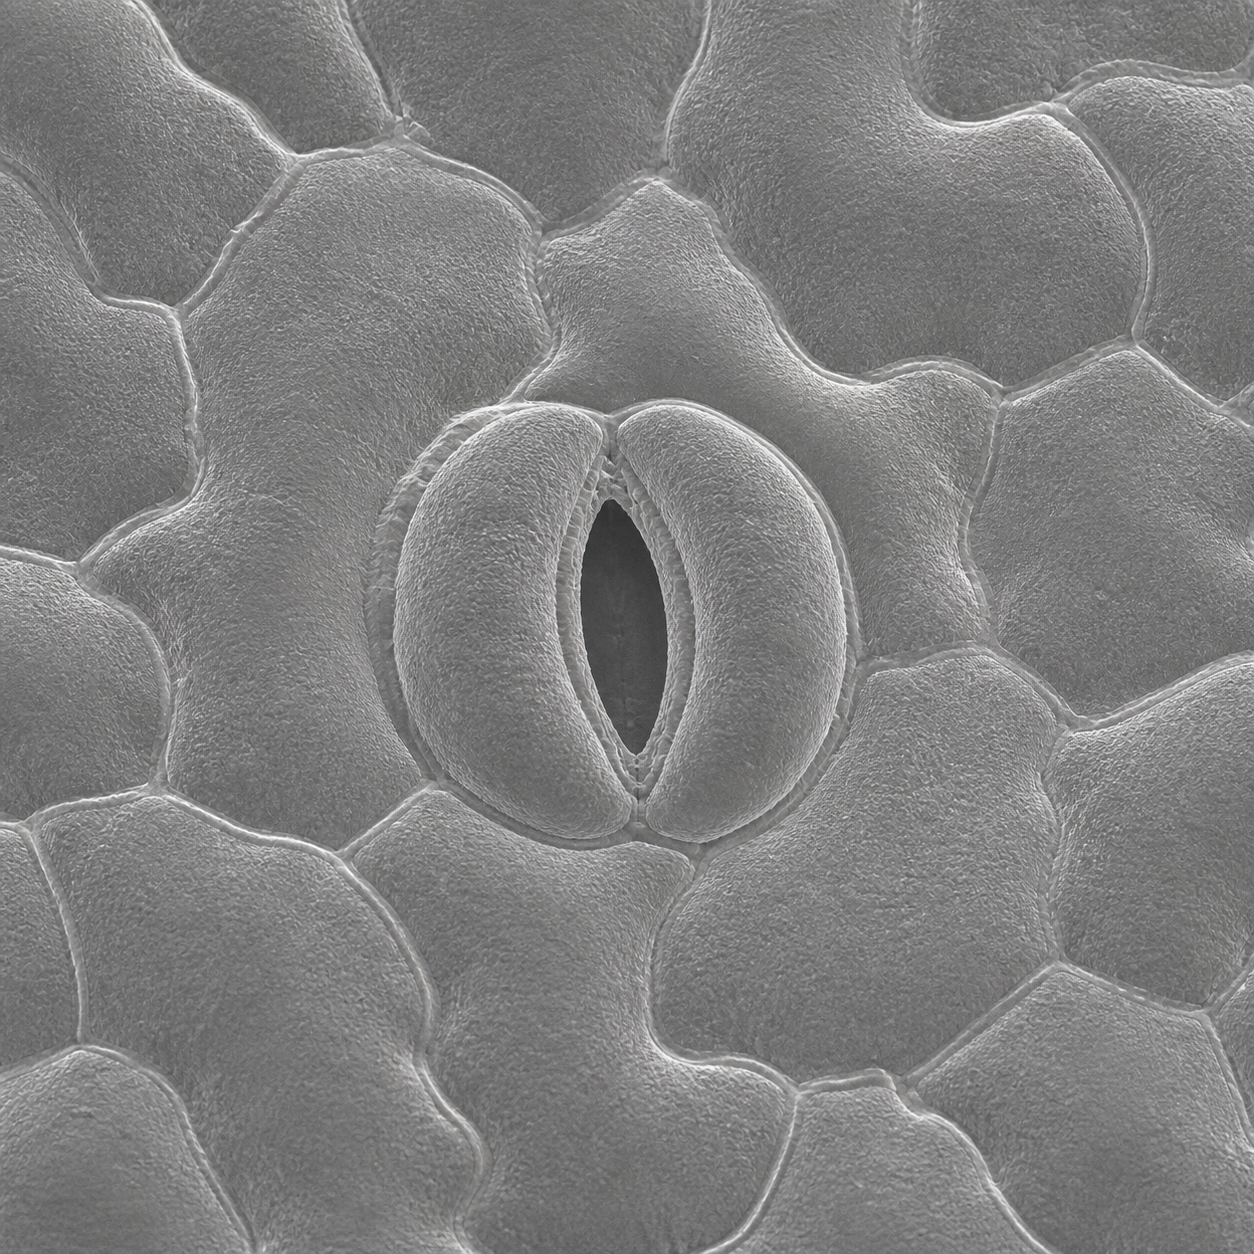
\includegraphics[width=0.4\linewidth]{images/book2/ai/g12-plant-stoma-sem.png}

{\small क्रमवीक्षी इलेक्ट्रॉन सूक्ष्मदर्शी से देखा गया एक \omterm{def:g12:plant-rooted-life:stomata}{रंध्र}: उस छिद्र के
चारों ओर दो गुर्दे जैसी रक्षक \omterm{def:g10:cells-common-unit:cell}{कोशिकाएँ}, पत्ते की खाल की चपटी \omterm{def:g10:cells-common-unit:cell}{कोशिकाओं} के
बीच। वह छिद्र कुछ ही माइक्रोमीटर चौड़ा है।}
\end{omfigure}

\begin{omfigure}
\begin{tikzpicture}
\begin{axis}[
  width=0.86\linewidth, height=5.4cm,
  axis x line=bottom, axis y line=left,
  xmin=0, xmax=24, ymin=0, ymax=110,
  xlabel={दिन का घंटा}, ylabel={अधिकतम का \%},
  xlabel style={font=\small, at={(axis description cs:0.5,-0.12)}, anchor=north},
  ylabel style={font=\small},
  tick label style={font=\small}, xtick={0,6,12,18,24}, ytick={0,50,100},
  legend style={at={(0.5,-0.3)}, anchor=north, legend columns=3, font=\small, draw=none},
]
\addplot[thick, omProp, smooth] coordinates {(0,0) (5,0) (6,20) (8,80) (12,100) (16,80) (19,20) (20,0) (24,0)};
\addplot[thick, omMeth, smooth] coordinates {(0,5) (5,5) (7,60) (9,95) (13,90) (15,40) (17,70) (19,30) (20,5) (24,5)};
\addplot[thick, omDef, dashed, smooth] coordinates {(0,3) (5,3) (7,50) (9,85) (13,100) (15,45) (17,65) (19,25) (20,3) (24,3)};
\legend{प्रकाश, रंध्रों का खुलना, वाष्पोत्सर्जन}
\end{axis}
\end{tikzpicture}

{\small किसी पत्ते का एक गर्मी का दिन। \omterm{def:g12:plant-rooted-life:stomata}{रंध्र} प्रकाश के साथ खुलते हैं और रात
में बंद हो जाते हैं; किसी गर्म दोपहर बाद वे पानी का नुक़सान सीमित करने के
लिए आंशिक रूप से बंद होते हैं, और वाष्पोत्सर्जन --- जो उनके खुलने के पीछे
चलता है --- उनके साथ नीचे बैठ जाता है।}
\end{omfigure}

\section{बिना किसी हृदय के पानी और भोजन चलाना}

\begin{proposition}[दो रस]\label{prop:g12:plant-rooted-life:saps}
किसी पौधे में परिवहन के दो तंत्र हैं, और दोनों हर अंग की शिराओं में नलियों
में जुड़ी लंबी \omterm{def:g10:cells-common-unit:cell}{कोशिकाओं} से बने हैं।
\begin{itemize}
  \item \emph{जाइलम}\index{जाइलम} \emph{कच्चा रस} --- यानी जड़ों का सोखा
        पानी तथा खनिज आयन --- ऊपर पत्तों तक ढोता है। चलाने वाला बल
        वाष्पोत्सर्जन है: पत्ते की \omterm{def:g10:cells-common-unit:cell}{कोशिकाओं} से वाष्पित होता पानी \omterm{prop:g12:plant-rooted-life:saps}{जाइलम} में
        पानी के लगातार स्तंभ को जड़ों से ऊपर खींचता है, जैसे कोई बत्ती तेल
        खींचती है। कोई पंप नहीं, पौधे की ख़र्च की गई कोई ऊर्जा नहीं: वह
        उठाई सूरज करता है।
  \item \emph{फ्लोएम}\index{फ्लोएम} \emph{निर्मित रस} --- यानी पत्तों के
        बनाए शर्करा वाला पानी --- पत्तों से हर उस अंग तक ढोता है जो उन्हें
        खपाता या जमा करता है: बढ़ते सिरे, जड़ें, फल, बीज, कंद। वह स्रोत से
        गर्त की ओर बहता है, और वह भी जिस भी दिशा में वे गर्त पड़े हों।
\end{itemize}
\end{proposition}
\begin{proof}[साक्ष्य]
रंगे पानी में रखा कोई कटा तना उस रंग को \omterm{prop:g12:plant-rooted-life:saps}{जाइलम} में चढ़ता दिखाता है, और किसी
थैले में बंद प्ररोह के मुक़ाबले वाष्पोत्सर्जन करते प्ररोह में तेज़ी से; और
जिस प्ररोह के पत्ते हटा दिए गए हों वह कुछ भी नहीं उठाता। किसी तने से छाल का
एक छल्ला (जिसमें \omterm{prop:g12:plant-rooted-life:saps}{फ्लोएम} होता है) हटा देने पर शर्करा जड़ों तक पहुँचनी बंद हो
जाती है, जो महीनों में भूखी मर जाती हैं, जबकि उस छल्ले के ऊपर के पत्तों को
पानी मिलता रहता है; शर्करा उस छल्ले के ऊपर जमा हो जाती है और छाल फूल जाती
है। \omterm{prop:g12:plant-rooted-life:saps}{फ्लोएम} पर अपने सुई जैसे मुँहों से खाते माहू, जब उस सुई से काट दिए जाएँ,
दाब में शर्करा भरे रस की एक बूँद देते हैं।
\end{proof}

\begin{omfigure}
\begin{tikzpicture}[font=\small, >=Stealth, line cap=round]
  % plant: roots, stem, leaves, fruit
  \draw[line width=6pt, omProp!40] (0,0) -- (0,5.5);           % stem
  \draw[thick, fill=omMeth!40] (0,4.6) .. controls (-1.2,5.0) and (-1.6,4.0) .. (-0.2,3.9) -- cycle;   % left leaf
  \draw[thick, fill=omMeth!40] (0,3.4) .. controls (1.2,3.8) and (1.6,2.8) .. (0.2,2.7) -- cycle;      % right leaf
  \draw[thick, fill=omThm!40] (0.9,5.4) circle (0.35);                                                 % fruit
  \draw[thick, omProp!60] (0,5.5) -- (0.7,5.3);
  \foreach \a in {-150,-120,-90,-60,-30} \draw[thick, omProp!70] (0,0) -- (\a:1.8);                   % roots
  \node[anchor=north] at (0,-1.9) {जड़ें: पानी और खनिज सोखती हैं};
  % xylem arrow (up)
  \draw[->, very thick, omDef] (-0.4,-1.2) -- (-0.4,4.4);
  \node[omDef, anchor=east, align=right] at (-0.6,1.5) {कच्चा रस: पानी\\ और खनिज,\\ वाष्पोत्सर्जन से\\ ऊपर खींचे गए};
  % phloem arrows (from leaves down and up)
  \draw[->, very thick, omThm] (0.4,3.0) -- (0.4,0.0) -- (0.4,-1.0);
  \draw[->, very thick, omThm] (0.4,3.6) -- (0.4,5.2) -- (0.75,5.2);
  \node[omThm, anchor=west, align=left] at (0.7,1.2) {निर्मित रस:\\ पत्तों से जड़ों,\\ फलों, बढ़ते सिरों\\ तक शर्करा};
  \draw[->, thick, gray] (-2.4,4.6) -- (-1.6,4.6) node[pos=0, left, align=right, font=\scriptsize] {जलवाष्प पत्ते\\ से निकलती है};
  \draw[<-, thick, gray] (-1.7,4.2) -- (-2.5,4.2);
\end{tikzpicture}

{\small वे दो बहाव। कच्चा रस \omterm{prop:g12:plant-rooted-life:saps}{जाइलम} में जड़ से पत्ते तक चढ़ता है, जिसे वह
पानी खींचता है जो \omterm{def:g12:plant-rooted-life:stomata}{रंध्रों} से वाष्पित होता है; और निर्मित रस \omterm{prop:g12:plant-rooted-life:saps}{फ्लोएम} में
पत्तों से वहाँ-वहाँ जाता है जहाँ शर्करा इस्तेमाल या जमा होती है --- नीचे
जड़ों तक, ऊपर किसी फल तक।}
\end{omfigure}

\begin{example}[किसी पेड़ के आँकड़े]\label{ex:g12:plant-rooted-life:numbers}
गर्मी के किसी दिन कोई पूरा बढ़ा भोजपत्र \qtyrange{300}{400}{L} पानी
वाष्पोत्सर्जित करता है, जो एक मिलीमीटर के दसवें हिस्से भर चौड़ी \omterm{prop:g12:plant-rooted-life:saps}{जाइलम}
नलियों से होकर \qty{20}{m} ऊपर, \qtyrange{1}{5}{m} प्रति घंटा की रफ़्तार से
उठाया जाता है। उस पानी का 1\% से भी कम \omterm{def:g10:cell-metabolism:autotrophy}{प्रकाशसंश्लेषण} के लिए रखा जाता है;
बाक़ी खुले \omterm{def:g12:plant-rooted-life:stomata}{रंध्रों} की क़ीमत है। बदले में वे पत्ते कोई \qty{5}{kg} कार्बन
डाइऑक्साइड को \qty{3.5}{kg} शर्करा में बाँध देते हैं, जिसका एक हिस्सा
\omterm{prop:g12:plant-rooted-life:saps}{फ्लोएम} हर जड़-सिरे और हर पकते बीज तक पहुँचाता है।
\end{example}

\section{अपनी ज़मीन पर डटे रहना}

\begin{proposition}[किसी जड़ जमाए जीव के बचाव]\label{prop:g12:plant-rooted-life:defences}
भाग न सकने के कारण पौधे अपनी जगह पर ही अपना बचाव करते हैं।
\begin{itemize}
  \item \emph{रचनाएँ}: सूखने तथा संक्रमण के ख़िलाफ़ मोम वाली उपत्वचा और
        छाल; शाकभक्षियों के ख़िलाफ़ काँटे, शूल, डंक मारते रोम और सिलिका;
        और हर \omterm{def:g10:cells-common-unit:cell}{कोशिका} में सेल्युलोज़ की एक मोटी दीवार।
  \item \emph{रसायन}: पत्तों को अपाच्य बनाते टैनिन, कड़वे क्षाराभ (कैफ़ीन,
        निकोटीन, मॉर्फ़ीन), विष, राल और वह क्षीर जो घाव बंद करता तथा कीटों
        को ज़हर देता है; इनमें से कई किसी हमले के बाद ही बनाए जाते हैं, और
        कुछ ऐसे उड़नशील संकेतों की तरह छोड़े जाते हैं जो पड़ोसी पत्तों को
        चेताते हैं तथा हमलावर कीट के शिकारियों को बुलाते हैं।
  \item \emph{सहनशीलता और नवीकरण}: हर गाँठ पर बढ़त के बिंदु, ताकि चरा गया
        प्ररोह दोबारा उग आए; सर्दी या सूखे भर सुप्ति; और ऐसे बीज जो
        मिट्टी में सालों इंतज़ार करते हैं।
\end{itemize}
\end{proposition}
\admitted

\begin{example}[किसी इल्ली का भोजन, और उसका जवाब]\label{ex:g12:plant-rooted-life:caterpillar}
किसी इल्ली के पहले कौरों के घंटों के भीतर कोई टमाटर का पौधा अपने पत्तों भर
ऐसे \omterm{def:g11:gene-expression:protein}{प्रोटीन} बनाता है जो उस कीट के पाचक \omterm{def:g11:enzymes-and-phenotype:enzyme}{एंजाइम} रोक देते हैं; और एक दिन के
भीतर हवा में छोड़ा उसका एक रसायन किसी परजीवी ततैया को उस इल्ली तक खींच लाता
है। वही हवाई संकेत पाते पड़ोसी टमाटर के पौधे किसी इल्ली के उन तक पहुँचने से
पहले ही पाचन रोकने वाले बनाने लगते हैं। वह पौधा हिलता नहीं, पर वह न
बेबस है और न अकेला।
\end{example}

\section{की ओर बढ़ना, से दूर बढ़ना}

\begin{proposition}[बढ़त ही हलचल]\label{prop:g12:plant-rooted-life:tropisms}
कोई पौधा बढ़कर हिलता है। उसके प्ररोह प्रकाश की ओर और गुरुत्व के ख़िलाफ़
बढ़ते हैं, और उसकी जड़ें गुरुत्व तथा पानी की ओर: यानी
\emph{अनुवर्तन}\index{अनुवर्तन}, जो दिशा वाली बढ़त प्रतिक्रियाएँ हैं। इन्हें
\omterm{def:g11:hormones-and-reproduction:hormone}{हॉर्मोन} नियंत्रित करते हैं, जिनमें सबसे पहले पहचाना गया \emph{ऑक्सिन} किसी
प्ररोह के बढ़ते सिरे में बनता है और तने से नीचे ढोया जाता है; और जिन
\omterm{def:g10:cells-common-unit:cell}{कोशिकाओं} को अधिक ऑक्सिन मिले वे अधिक लंबी होती हैं। किसी प्ररोह के एक ओर
पड़ता प्रकाश उस ऑक्सिन को छाया वाली ओर खिसका देता है, जो तेज़ी से बढ़कर उस
प्ररोह को प्रकाश की ओर मोड़ देती है।
\end{proposition}
\begin{proof}[साक्ष्य]
एक ओर से रोशन घास के नन्हे पौधे प्रकाश की ओर मुड़ते हैं; सिरे पर ढँके हों तो
नहीं मुड़ते, हालाँकि मुड़ने वाला हिस्सा नीचे है; और केवल आधार पर ढँके हों तो
वे सामान्य ढंग से मुड़ते हैं: यानी सिरा भाँपता है, आधार जवाब देता है, और
उनके बीच कोई चीज़ चलती है। कोई सिरा काटकर जेल के किसी टुकड़े पर रखा जाए,
फिर वह जेल किसी सिर-कटे नन्हे पौधे की एक ओर रखा जाए, तो वह अँधेरे में उस
टुकड़े से दूर मुड़ जाता है --- यानी उस जेल में बैठी चीज़, ऑक्सिन, अपने आप
में काफ़ी है। सीधे नापने पर किसी रोशन नन्हे पौधे की छाया वाली ओर रोशन ओर से
लगभग दुगना ऑक्सिन थामे रहती है।
\end{proof}

\begin{omfigure}
\begin{tikzpicture}[font=\small, >=Stealth, line cap=round]
  \tikzset{seedling/.style={line width=4pt, omMeth!70}}
  % light source arrow
  \foreach \x in {0,3.6,7.2,10.8} \draw[->, thick, omProp] (\x-1.4,2.2) -- (\x-0.6,2.2);
  \node[omProp, anchor=east, font=\scriptsize] at (-1.5,2.2) {प्रकाश};
  % 1: intact, bends toward light
  \draw[seedling] (0,0) -- (0,1.6) .. controls (0,2.2) .. (-0.5,2.6);
  \node[anchor=north, align=center] at (0,-0.2) {अछूता:\\ प्रकाश की ओर मुड़ता};
  % 2: tip covered: no bending
  \draw[seedling] (3.6,0) -- (3.6,2.7);
  \draw[fill=black] (3.4,2.4) rectangle (3.8,2.9);
  \node[anchor=north, align=center] at (3.6,-0.2) {सिरा ढँका:\\ कोई मोड़ नहीं};
  % 3: base covered: bends
  \draw[seedling] (7.2,0) -- (7.2,1.6) .. controls (7.2,2.2) .. (6.7,2.6);
  \draw[fill=black!60, opacity=0.5] (6.95,0) rectangle (7.45,1.3);
  \node[anchor=north, align=center] at (7.2,-0.2) {आधार ढँका:\\ प्रकाश की ओर मुड़ता};
  % 4: tip removed: no bending
  \draw[seedling] (10.8,0) -- (10.8,2.2);
  \draw[thick] (10.5,2.35) -- (11.1,2.35);
  \node[anchor=north, align=center] at (10.8,-0.2) {सिरा हटाया:\\ कोई मोड़ नहीं};
\end{tikzpicture}

{\small नन्हे पौधों के प्रकाश की ओर मुड़ने पर वे शास्त्रीय प्रयोग। सिरा
प्रकाश भाँपता है; उसके नीचे का हिस्सा मुड़ने का काम करता है; और एक संकेत ---
ऑक्सिन --- एक से दूसरे तक जाता है।}
\end{omfigure}

\section{बिना हिले जनन करना}

\begin{proposition}[फूल और उनके मेहमान]\label{prop:g12:plant-rooted-life:flowers}
\emph{फूल} अधिकांश थलीय पौधों का जननांग है: \emph{पुंकेसर}, जो पराग यानी उस
पौधे के नर युग्मक बनाते हैं, और कोई \emph{स्त्रीकेसर}, जिसके बीजांड मादा
युग्मक थामते हैं। चूँकि कोई भी जनक हिलता नहीं, इसलिए पराग को एक फूल से दूसरे
तक ढोया जाना चाहिए --- घासों और बहुत-से पेड़ों के मामले में हवा से, जिनके
छोटे, फीके फूल लाखों की गिनती में पराग झाड़ते हैं, या अधिकांश फूल वाले
पौधों के मामले में जंतुओं से, जिनकी पंखुड़ियाँ, गंध और मकरंद उन कीटों,
पक्षियों तथा चमगादड़ों को दी गई क़ीमत हैं जो खाते-खाते पराग ढो ले जाते हैं।
फूल और परागणकर्ता अक्सर साथ-साथ विकसित हुए हैं, और हर एक दूसरे के आकार तथा
आदतों के अनुकूल है।
\end{proposition}
\admitted

\begin{example}[मेल खाते आकार]\label{ex:g12:plant-rooted-life:match}
मकरंद की \qty{30}{cm} नली वाले किसी फूल पर \qty{30}{cm} जीभ वाला कोई शलभ
आता है, और उसके अलावा कुछ भी नहीं; दिन में खुला कोई लाल, गंधहीन, नलीदार फूल
किसी पक्षी का फूल है; भारी गंध के साथ रात में खुलता कोई फीका फूल किसी शलभ का;
और उतरने के मंच वाला पीली पंखुड़ियों का कोई कटोरा किसी मधुमक्खी का। वह पौधा
ऐसी सेवा के लिए शर्करा में क़ीमत चुकाता है जो वह ख़ुद नहीं कर सकता, और उस
परागणकर्ता का विशेषीकरण पक्का करता है कि वह पराग उसी \omterm{def:g10:biodiversity-scales:species}{जाति} के किसी दूसरे फूल
तक जाए।
\end{example}

\begin{proposition}[फल और प्रकीर्णन]\label{prop:g12:plant-rooted-life:dispersal}
निषेचन के बाद वह बीजांड एक \emph{बीज} बनता है --- यानी किसी सुरक्षा कवच में
बैठा, सुप्त, भोजन भंडार वाला एक भ्रूण --- और वह स्त्रीकेसर एक \emph{फल}, जो
उन बीजों को जनक से दूर ले जाता है: पंखों तथा गुच्छों से हवा पर; पानी से;
अँकुड़ों से जंतुओं की खाल पर; और जंतुओं के भीतर, जब कोई गूदेदार फल खाया जाता
है और उसके बीज कहीं और, बिना किसी चोट के, खाद की एक ख़ुराक के साथ गिराए
जाते हैं। बीज उस पौधे की इकलौती गतिशील अवस्था है और इंतज़ार करने का उसका
इकलौता ज़रिया: वह किलोमीटर चल सकता है और साल सो सकता है।
\end{proposition}
\admitted

\begin{method}[जड़ जमाए जीवन के किसी अनुकूलन को पढ़ना]\label{met:g12:plant-rooted-life:read}
किसी पौधे की किसी भी विशेषता के लिए पूछिए:
\begin{enumerate}
  \item वह किसी नियत जीव की कौन-सी ज़रूरत पूरी करती है --- प्रकाश या
        कार्बन डाइऑक्साइड पकड़ना, पानी सोखना, ढोना, बचाव करना, दिशा लेना,
        पराग या बीज बिखेरना?
  \item वह कौन-सी सतह, रचना या पदार्थ इस्तेमाल करती है, और किस क़ीमत पर
        (\omterm{def:g12:plant-rooted-life:stomata}{रंध्रों} से खोया पानी, मकरंद या विषों पर ख़र्च ऊर्जा)?
  \item क्या उसमें कोई दूसरा जीव शामिल है (परागणकर्ता, बिखेरने वाला, जड़ का
        कवक, शाकभक्षी), और हर साझीदार को क्या मिलता है?
  \item क्या वह एक ही बार बनी है (छाल, काँटे) या माँग पर बनाई जाती है
        (हमले के बाद कोई विष, प्रकाश की ओर कोई मोड़)?
\end{enumerate}
\end{method}

\begin{remark}[जीवन का आधा हिस्सा, खड़े-खड़े]\label{rem:g12:plant-rooted-life:half}
पृथ्वी के जीवित द्रव्यमान का अधिकांश पौधे बनाते हैं और बाक़ी लगभग सबको
खिलाते हैं। \omterm{def:g10:cell-metabolism:autotrophy}{प्रकाशसंश्लेषण} तथा श्वसन पर आगे आते अध्याय उनका रसायन बताते हैं;
और इसने वह देह बताई है जो उसे चलाती है: एक नियत बिंदु, जहाँ से सतहें मिट्टी
तथा हवा में फैलती हैं, रस बिना किसी पंप के बहते हैं, उड़ान की जगह रसायन आ
जाता है, हलचल की जगह बढ़त, और सफ़र के लिए जंतु काम पर रखे जाते हैं।
\end{remark}

\section{अभ्यास}

\begin{exercise}[$\star$]\label{exo:g12:plant-rooted-life:1}
किसी फूल वाले पौधे के दोनों तंत्रों का और हर एक की लेन-देन सतह का नाम
लीजिए।
\end{exercise}

\begin{exercise}[$\star$]\label{exo:g12:plant-rooted-life:2}
\omterm{def:g12:plant-rooted-life:stomata}{रंध्र} क्या है, हर दिशा में उससे होकर क्या गुज़रता है, और वह कब खुला रहता
है?
\end{exercise}

\begin{exercise}[$\star$]\label{exo:g12:plant-rooted-life:3}
कच्चे रस को निर्मित रस से अलग कीजिए: सामग्री, नलियाँ, दिशा, चलाने वाला बल।
\end{exercise}

\begin{exercise}[$\star$]\label{exo:g12:plant-rooted-life:4}
पौधों के दो रचनात्मक और दो रासायनिक बचाव दीजिए।
\end{exercise}

\begin{exercise}[$\star$]\label{exo:g12:plant-rooted-life:5}
\omterm{prop:g12:plant-rooted-life:tropisms}{अनुवर्तन} क्या है? किसी प्ररोह के प्रकाश की ओर मुड़ने को कौन-सा \omterm{def:g11:hormones-and-reproduction:hormone}{हॉर्मोन}
नियंत्रित करता है, और वह कहाँ बनता है?
\end{exercise}

\begin{exercise}[$\star\star$]\label{exo:g12:plant-rooted-life:6}
\qty{40}{cm^2} का कोई पत्ता अपनी निचली सतह पर प्रति वर्ग मिलीमीटर 200 \omterm{def:g12:plant-rooted-life:stomata}{रंध्र}
ढोता है। उसमें कितने \omterm{def:g12:plant-rooted-life:stomata}{रंध्र} हैं? और 200\,000 पत्तों वाले किसी पेड़ पर कितने?
\end{exercise}

\begin{exercise}[$\star\star$]\label{exo:g12:plant-rooted-life:7}
गर्मी के दिन वाले चित्र से बताइए कि वाष्पोत्सर्जन किस घंटे सबसे अधिक है, और
वह दोपहर बाद क्यों नीचे बैठता है जबकि प्रकाश नहीं बैठता।
\end{exercise}

\begin{exercise}[$\star\star$]\label{exo:g12:plant-rooted-life:8}
वसंत में किसी तने के चारों ओर से छाल का एक छल्ला हटा दिया जाता है। अनुमान
लगाइए कि आगे के महीनों में पत्तों, जड़ों और उस छल्ले के ठीक ऊपर की छाल का
क्या होगा।
\end{exercise}

\begin{exercise}[$\star\star$]\label{exo:g12:plant-rooted-life:9}
नन्हे पौधे वाले चित्र में समझाइए कि चारों प्रयोगों में से हर एक क्या
स्थापित या ख़ारिज करता है, और चारों क्यों ज़रूरी हैं।
\end{exercise}

\begin{exercise}[$\star\star$]\label{exo:g12:plant-rooted-life:10}
कोई पौधा हर दिन \qty{300}{L} पानी अपने पत्तों तक उठाता है और उस पर कोई
ऊर्जा ख़र्च नहीं करता। समझाइए कि वह ऊर्जा कहाँ से आती है।
\end{exercise}

\begin{exercise}[$\star\star$]\label{exo:g12:plant-rooted-life:11}
हवा से परागित और कीट से परागित फूल की चार बिंदुओं पर तुलना कीजिए, और हर
अंतर को उस ढोने वाले से समझाइए।
\end{exercise}

\begin{exercise}[$\star\star\star$]\label{exo:g12:plant-rooted-life:12}
कोई पौधा सूखे के दौरान अपने \omterm{def:g12:plant-rooted-life:stomata}{रंध्र} बंद कर लेता है। समझाइए कि उसे क्या मिलता
है, क्या खोता है, और कोई लंबा सूखा उसे तब भी क्यों मार डालता है जब वह पानी
खोना बंद कर चुका है।
\end{exercise}

\begin{exercise}[$\star\star\star$]\label{exo:g12:plant-rooted-life:13}
कैफ़ीन कॉफ़ी के किसी पत्ते वाली ख़ुराकों पर कीटों के लिए विषैली है पर
मकरंद में उसकी दसवें हिस्से भर ख़ुराक में मौजूद है, जहाँ वह उस फूल के प्रति
मधुमक्खियों की याददाश्त सुधारती है। इसे \cref{met:g12:plant-rooted-life:read}
से पढ़िए: वही अणु उन दोनों जगहों पर क्या करता है?
\end{exercise}

\begin{exercise}[$\star\star\star$]\label{exo:g12:plant-rooted-life:14}
\qty{30}{cm} मकरंद नली वाले किसी फूल का इकलौता परागणकर्ता \qty{30}{cm} जीभ
वाला कोई शलभ है। समझाइए कि ऐसा मेल क़दम-दर-क़दम कैसे विकसित हो सकता है, और
दूसरा ग़ायब हो जाए तो हर साझीदार क्या जोखिम उठाता है।
\end{exercise}

\begin{exercise}[$\star\star\star$]\label{exo:g12:plant-rooted-life:15}
``पौधा एक निष्क्रिय जीव है।'' इस वाक्य को एक अनुच्छेद में सही ढंग से दोबारा
लिखिए, और उसमें भाँपने, जवाब देने, बचाव करने तथा भर्ती करने का एक-एक उदाहरण
दीजिए।
\end{exercise}

\section{समस्या: किसी बलूत का गर्मी का दिन}

\begin{problem}[{सप्ताहांत समस्या --- किसी पेड़ के लेन-देन का हिसाब: पत्ते
और रंध्र गिने गए, पानी उठाया गया और शर्करा बनाई गई, फ्लोएम की सप्लाई, और
बाहर भेजे गए बीज}]
\label{pb:g12:plant-rooted-life:1}
कोई पूरा बढ़ा बलूत \qty{25}{cm^2} के 250\,000 पत्ते ढोता है। उसकी निचली
पत्ती सतहें प्रति वर्ग मिलीमीटर 250 \omterm{def:g12:plant-rooted-life:stomata}{रंध्र} रखती हैं। गर्मी के किसी दिन पत्ती
का हर वर्ग मीटर \qty{0.6}{L} पानी वाष्पोत्सर्जित करता है और \qty{8}{g}
कार्बन डाइऑक्साइड शर्करा में बाँधता है। पत्ते 90\% पानी हैं; और
\omterm{def:g10:cell-metabolism:autotrophy}{प्रकाशसंश्लेषण} बनाई गई हर \qty{1.6}{g} शर्करा पर \qty{1}{g} पानी इस्तेमाल
करता है।

\medskip
\noindent\textbf{भाग I --- सतहें।}
\begin{enumerate}
  \item उस बलूत का कुल पत्ती क्षेत्रफल वर्ग मीटरों में निकालिए।
  \item उस पेड़ पर \omterm{def:g12:plant-rooted-life:stomata}{रंध्रों} की संख्या निकालिए।
  \item उस पेड़ का शिखर \qty{150}{m^2} ज़मीन ढँकता है। ज़मीन के हर वर्ग
        मीटर के ऊपर पत्ती के कितने वर्ग मीटर चिने हुए हैं?
  \item ऐसे किसी पेड़ के \omterm{prop:g12:plant-rooted-life:surfaces}{मूलरोम} मिट्टी के सामने लगभग \qty{1000}{m^2} पेश
        करते हैं। पत्तों से तुलना कीजिए और समझाइए कि दोनों सतहें एक ही
        कोटि की क्यों हैं।
  \item पत्ती सतह को किसी एक मोटे अंग में सिमटाने के बजाय पतला फैलाकर चिना
        क्यों जाना चाहिए?
\end{enumerate}

\medskip
\noindent\textbf{भाग II --- पानी।}
\begin{enumerate}[resume]
  \item उस दिन बलूत के वाष्पोत्सर्जित पानी का आयतन निकालिए।
  \item बनाई गई शर्करा का द्रव्यमान, और उसे बनाने में इस्तेमाल हुए पानी का
        द्रव्यमान निकालिए। वह वाष्पोत्सर्जित पानी का कौन-सा अंश है?
  \item समझाइए कि वह पेड़ बाक़ी क्यों नहीं रख सकता: वह उसे बचाने के लिए
        अपने \omterm{def:g12:plant-rooted-life:stomata}{रंध्र} बंद कर ले तो क्या होगा?
  \item वह पानी \omterm{prop:g12:plant-rooted-life:saps}{जाइलम} से होकर \qty{20}{m} ऊपर चढ़ता है। ऊर्जा कौन जुटाता
        है, और पेड़ के अपने किसी पंप की उसे क्या क़ीमत पड़ती?
  \item किसी गर्म, सूखी दोपहर बाद वाष्पोत्सर्जन गिरकर एक तिहाई रह जाता है
        जबकि प्रकाश अपने अधिकतम पर है। उस पेड़ ने क्या किया है, और उसकी
        शर्करा में क्या क़ीमत पड़ती है?
\end{enumerate}

\medskip
\noindent\textbf{भाग III --- शर्करा।}
उस बलूत की जड़ें, तना और बढ़ते प्ररोह श्वसन तथा बढ़त में हर दिन \qty{2}{kg}
शर्करा खपाते हैं; और उसके बलूत-फल अपने मौसम में और \qty{0.5}{kg} लेते हैं।
\begin{enumerate}[resume]
  \item उस दिन बनाई गई शर्करा और जड़ों, तने तथा प्ररोहों को और बलूत-फलों को
        पहुँचाया गया अंश निकालिए।
  \item कौन-सा ऊतक वह शर्करा ढोता है, और किससे किस तक?
  \item बची हुई शर्करा का क्या होता है, और वह अगले वसंत कहाँ मिल सकती है?
  \item जून में छाल का एक छल्ला काटा जाता है। सवाल 11 के कौन-से आँकड़े
        बदलते हैं, और कैसे?
  \item समझाइए कि मई में अपने आधे पत्ते इल्लियों को खो देता कोई पेड़ मौसम
        अच्छा हो तो फिर भी बलूत-फल क्यों बना सकता है।
\end{enumerate}

\medskip
\noindent\textbf{भाग IV --- अगली पीढ़ी भेजना।}
वह बलूत हवा से परागित होता है और किसी अच्छे साल में 10\,000 बलूत-फल बनाता
है; जे पक्षी उनमें से लगभग 3000 ले जाकर गाड़ देते हैं, जिनमें से वे बाद में
अधिकांश खा जाते हैं; और गिलहरियाँ तथा चूहे बाक़ी लगभग सारे खा जाते हैं।
\begin{enumerate}[resume]
  \item हवा से परागण के चलते आप उस बलूत के फूलों की कौन-सी तीन विशेषताओं की
        उम्मीद करते हैं, गिनाइए।
  \item वह पेड़ जे पक्षियों को ऐसे बलूत-फलों में ``क़ीमत'' क्यों चुकाता है
        जो वह खो देगा, और उन्हें अपने ही नीचे क्यों नहीं गिरा देता?
  \item कोई जे पक्षी अपने गाड़े बलूत-फलों में से 5\% भूल जाए और गाड़े गए 50
        में से एक बलूत-फल कोई नवपौध बने, तो साल की उस फ़सल से कितने नवपौध
        मिलते हैं?
  \item वह बलूत 300 साल जीता है और उसे एक ही वयस्क पेड़ से बदला जाना है।
        अपने पिछले जवाब से तुलना कीजिए और समझाइए कि वे संख्याएँ क्यों ठीक
        बैठती हैं।
  \item परिणाम लिखिए: उस बलूत का पत्ती क्षेत्रफल और \omterm{def:g12:plant-rooted-life:stomata}{रंध्रों} की संख्या, वे
        लीटर जो वह अपनी बनाई किलोग्राम शर्करा के लिए एक दिन में उठाता है,
        और वे दो कारक जो उसके लिए हिलने का काम करते हैं।
\end{enumerate}
\end{problem}
